% !TEX root = morphkasten.tex

\section{Containererkennung (grob)}


%##############
\subsection{Sensor}

Grafik

\begin{table}[h]
\begin{tabular}{p{0.5\textwidth} | p{0.5\textwidth}}


 \textbf{Vorteile} & \textbf{Nachteile} \\ \hline
	 
\begin{itemize}
\item Vorteil 1
\item Vorteil 2
\item Vorteil 3
\item ...
\end{itemize}

 
 &
 
\begin{itemize}
\item Nachteil 1
\item Nachteil 2
\item Nachteil 3
\item ...
\end{itemize}

\end{tabular}
\end{table}

\begin{table}[h]
\begin{tabular}{p{0.5\textwidth}p{0.5\textwidth}}


 \textbf{Risiken} & \\ \hline
	 
\begin{itemize}
\item Risiko 1
\item Risiko 2
\end{itemize}
&
\begin{itemize}
\item Risiko 3
\item ...
\end{itemize}

 
\end{tabular}
\end{table}

\pagebreak


%##############
\subsection{Bilderkennung}
\begin{figure}[h!]%Position festigen
\centering
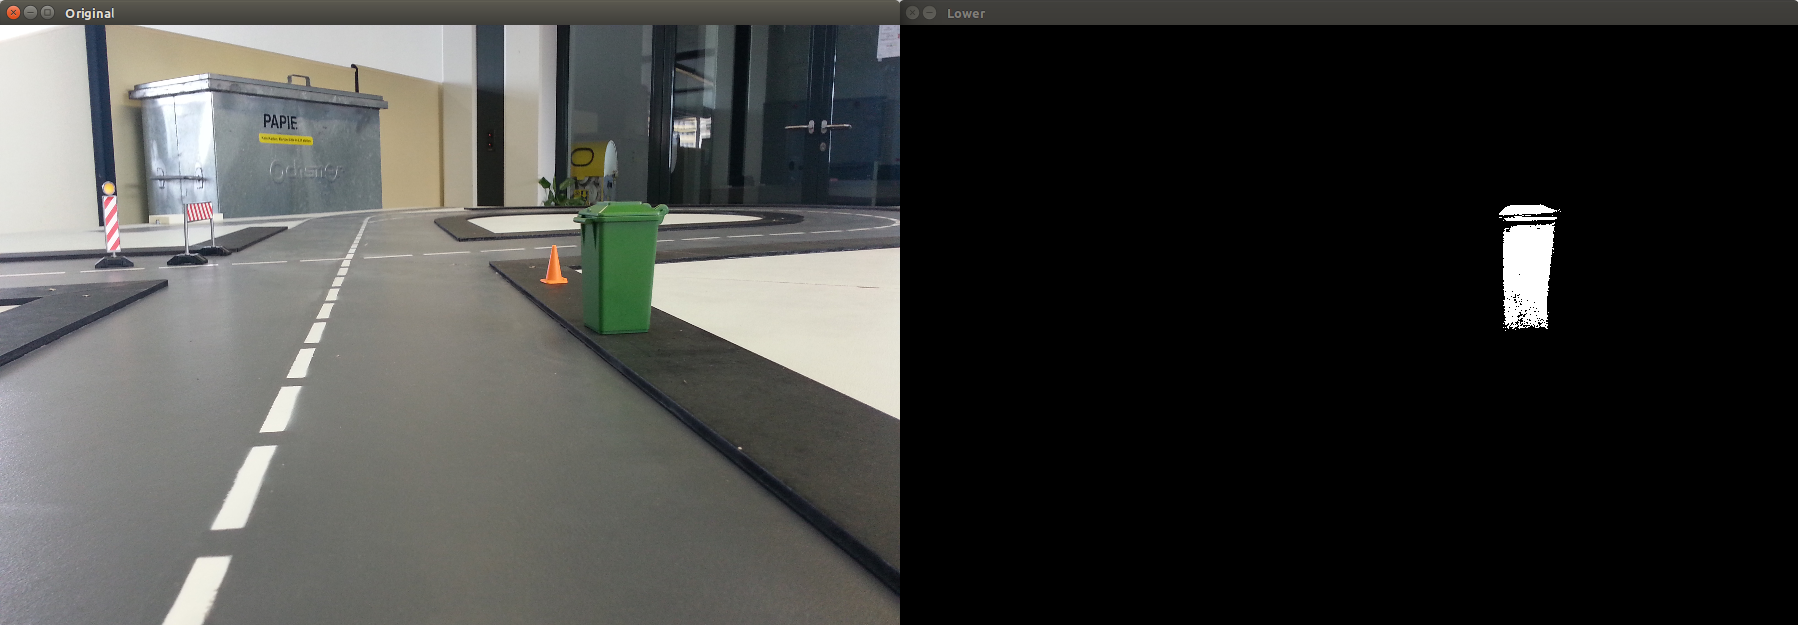
\includegraphics[width=0.7\textwidth]{fig/containererkennung_grob_bilderkennung.png}
\caption{Bilderkennung Container}
\label{fig:Bilderkennung Container}
\end{figure}

\begin{table}[h]
\begin{tabular}{p{0.5\textwidth} | p{0.5\textwidth}}


\textbf{Vorteile} & \textbf{Nachteile} \\ \hline
	 
\begin{itemize}
\item bei grösserer Distanz zu Container schon erkennbar
\item Containererkennung durch Form- und/oder Farberkennung
\end{itemize}

 
 &
 
\begin{itemize}
\item Algorithmus nötig
\item rechenintensiv
\end{itemize}

\end{tabular}
\end{table}

\begin{table}[h]
\begin{tabular}{p{0.5\textwidth}p{0.5\textwidth}}

\textbf{Risiken} & \\ \hline
	 
\begin{itemize}
\item bei verschiedene Lichtverhätlnissen variieren die Farben
\item Container kann zum Teil von anderen Gegeständen verdeckt sein
\end{itemize}

 
\end{tabular}
\end{table}

\pagebreak